\documentclass{beamer}

\usepackage{amssymb}
\usepackage{mathrsfs}
\usepackage{stmaryrd}
\usepackage{tikz-cd}


\newcommand{\CC}{\mathbb{C}}
\newcommand{\FF}{\mathbb{F}}
\newcommand{\NN}{\mathbb{N}}
\newcommand{\QQ}{\mathbb{Q}}
\newcommand{\RR}{\mathbb{R}}
\newcommand{\ZZ}{\mathbb{Z}}
\newcommand{\id}{\mathrm{id}}
\newcommand{\op}[1]{#1^{\text{op}}}
\newcommand{\powerset}[1]{\mathcal{P}(#1)}

\newcommand{\Set}{\mathbf{Set}}

%\renewcommand\labelenumii{(\roman{enumii})}

%\theoremstyle{definition}
%\newtheorem{theorem}{Theorem}[section]
%\newtheorem{proposition}[theorem]{Proposition}
%\newtheorem{definition}[theorem]{Definition}
%\newtheorem{lemma}[theorem]{Lemma}
%\newtheorem{corollary}[theorem]{Corollary}
%\newtheorem{example}{Example}[theorem]

\usetikzlibrary{backgrounds, intersections, calc}
\tikzstyle{dot}=[circle, draw=black, fill=black, minimum size=1mm, inner sep=0mm]
\tikzstyle{bg}=[gray!30]

\mode<presentation>
{
    %\usetheme{Warsaw}
}

\title{String diagrams}
\author{bpaul :3}
\date{\today}

\begin{document}

\begin{frame}
    \titlepage
\end{frame}

\begin{frame}
    \frametitle{Outline}
    \tableofcontents
\end{frame}

\section{The calculus of string diagrams}

\begin{frame}
    \frametitle{Our first diagrams}
    \begin{minipage}[t]{0.40\textwidth}
        \vspace*{0mm}
        \only<1-1>{
            
\begin{tikzpicture}[scale=2]
                 %Coordinate layout and vertex positioning
                \path
                    coordinate (bot)
                    +(0,1) coordinate[] (f)
                    +(0,2) coordinate (top);
                % Line drawing
                %\draw (bot) -- (top);
                % Region filling
                \begin{scope}[on background layer]
                \fill[bg] (bot -| -1,0) rectangle (top -| 1,0);
                \end{scope}
            \end{tikzpicture}
        }
        \only<2-2>{
            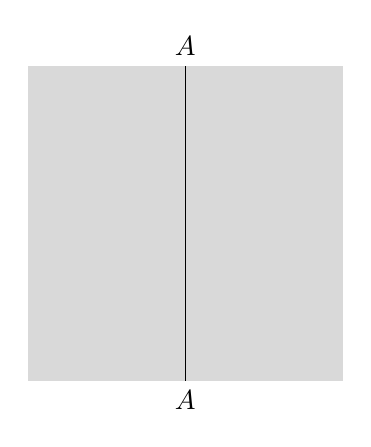
\begin{tikzpicture}[scale=2]
                 %Coordinate layout and vertex positioning
                \path
                    coordinate[label=below:\(A\)] (bot)
                    +(0,1) coordinate[] (f)
                    +(0,2) coordinate[label=above:\(A\)] (top);
                % Line drawing
                \draw (bot) -- (top);
                % Region filling
                \begin{scope}[on background layer]
                \fill[bg] (bot -| -1,0) rectangle (top -| 1,0);
                \end{scope}
            \end{tikzpicture}
        }
        \only<3-3>{
            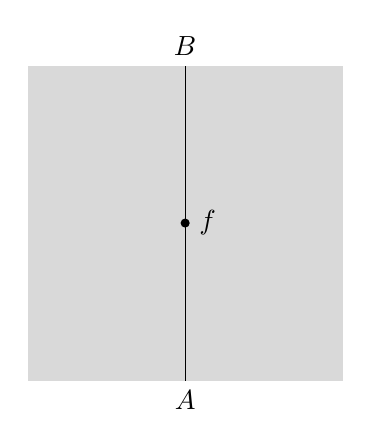
\begin{tikzpicture}[scale=2]
                 %Coordinate layout and vertex positioning
                \path
                    coordinate[label=below:\(A\)] (bot)
                    +(0,1) coordinate[dot, label=right:\(f\)] (f)
                    +(0,2) coordinate[label=above:\(B\)] (top);
                % Line drawing
                \draw (bot) -- (top);
                % Region filling
                \begin{scope}[on background layer]
                \fill[bg] (bot -| -1,0) rectangle (top -| 1,0);
                \end{scope}
            \end{tikzpicture}
        }
    \end{minipage}
    \begin{minipage}[t]{0.47\textwidth}
        \vspace*{5mm}
        \only<2-2>{
            Here \(A\) is a set.
        }
        \only<3-3>{
            Here \(A\) and \(B\) are sets, and \({f : A \to B}\) is a function.
        }
    \end{minipage}
\end{frame}

\begin{frame}
    \frametitle{Compositions}
    Vertical composition \(a \mapsto g(f(a))\):
    \begin{equation*}
        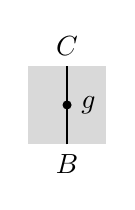
\begin{tikzpicture}[scale=0.5, baseline=($(top)!0.5!(bot)$)]
             %Coordinate layout and vertex positioning
            \path
                coordinate[label=below:\(B\)] (bot)
                +(0,1) coordinate[dot, label=right:\(g\)] (g)
                +(0,2) coordinate[label=above:\(C\)] (top);
            % Line drawing
            \draw (bot) -- (top);
            % Region filling
            \begin{scope}[on background layer]
            \fill[bg] (bot -| -1,0) rectangle (top -| 1,0);
            \end{scope}
        \end{tikzpicture}
        \circ
        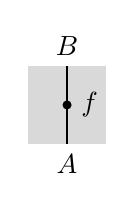
\begin{tikzpicture}[scale=0.5, baseline=($(top)!0.5!(bot)$)]
             %Coordinate layout and vertex positioning
            \path
                coordinate[label=below:\(A\)] (bot)
                +(0,1) coordinate[dot, label=right:\(f\)] (f)
                +(0,2) coordinate[label=above:\(B\)] (top);
            % Line drawing
            \draw (bot) -- (top);
            % Region filling
            \begin{scope}[on background layer]
            \fill[bg] (bot -| -1,0) rectangle (top -| 1,0);
            \end{scope}
        \end{tikzpicture}
        =
        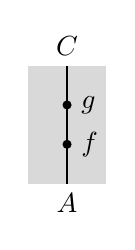
\begin{tikzpicture}[scale=0.5, baseline=($(top)!0.5!(bot)$)]
             %Coordinate layout and vertex positioning
            \path
                coordinate[label=below:\(A\)] (bot)
                +(0,1)coordinate[dot, label=right:\(f\)] (f)
                +(0,2)coordinate[dot, label=right:\(g\)] (g)
                +(0,3) coordinate[label=above:\(C\)] (top);
            % Line drawing
            \draw (bot) -- (top);
            % Region filling
            \begin{scope}[on background layer]
            \fill[bg] (bot -| -1,0) rectangle (top -| 1,0);
            \end{scope}
        \end{tikzpicture}
    \end{equation*}
    \pause
    Horizontal composition \((a, b) \mapsto (f(a), g(b))\):
    \begin{equation*}
        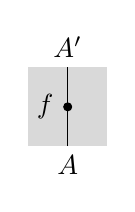
\begin{tikzpicture}[scale=0.5, baseline=($(top)!0.5!(bot)$)]
             %Coordinate layout and vertex positioning
            \path
                coordinate[label=below:\(A\)] (bot)
                +(0,1) coordinate[dot, label=left:\(f\)] (f)
                +(0,2) coordinate[label=above:\(A'\)] (top);
            % Line drawing
            \draw (bot) -- (top);
            % Region filling
            \begin{scope}[on background layer]
            \fill[bg] (bot -| -1,0) rectangle (top -| 1,0);
            \end{scope}
        \end{tikzpicture}
        \times
        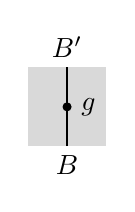
\begin{tikzpicture}[scale=0.5, baseline=($(top)!0.5!(bot)$)]
             %Coordinate layout and vertex positioning
            \path
                coordinate[label=below:\(B\)] (bot)
                +(0,1) coordinate[dot, label=right:\(g\)] (b)
                +(0,2) coordinate[label=above:\(B'\)] (top);
            % Line drawing
            \draw (bot) -- (top);
            % Region filling
            \begin{scope}[on background layer]
            \fill[bg] (bot -| -1,0) rectangle (top -| 1,0);
            \end{scope}
        \end{tikzpicture}
        =
        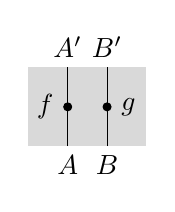
\begin{tikzpicture}[scale=0.5, baseline=($(dl)!0.5!(tl)$)]
             %Coordinate layout and vertex positioning
            \path
                coordinate[label=below:\(A\)] (dl)
                +(1,0)coordinate[label=below:\(B\)] (dr)
                +(0,1)coordinate[dot, label=left:\(f\)] (f)
                +(1,1)coordinate[dot, label=right:\(g\)] (g)
                +(0,2) coordinate[label=above:\(A'\)] (tl)
                +(1,2) coordinate[label=above:\(B'\)] (tr);
            % Line drawing
            \draw (dl) -- (tl);
            \draw (dr) -- (tr);
            % Region filling
            \begin{scope}[on background layer]
            \fill[bg] (dl -| -1,0) rectangle (tr -| 2,0);
            \end{scope}
        \end{tikzpicture}
    \end{equation*}
\end{frame}

\begin{frame}
    \frametitle{Rules}
    \begin{equation*}
        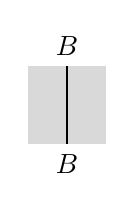
\begin{tikzpicture}[scale=0.5, baseline=($(bot)!0.5!(top)$)]
             %Coordinate layout and vertex positioning
            \path
                coordinate[label=below:\(B\)] (bot)
                +(0,1) coordinate[] (f)
                +(0,2) coordinate[label=above:\(B\)] (top);
            % Line drawing
            \draw (bot) -- (top);
            % Region filling
            \begin{scope}[on background layer]
            \fill[bg] (bot -| -1,0) rectangle (top -| 1,0);
            \end{scope}
        \end{tikzpicture}
        \circ
        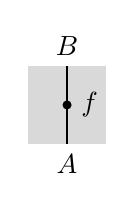
\begin{tikzpicture}[scale=0.5, baseline=($(bot)!0.5!(top)$)]
             %Coordinate layout and vertex positioning
            \path
                coordinate[label=below:\(A\)] (bot)
                +(0,1) coordinate[dot, label=right:\(f\)] (f)
                +(0,2) coordinate[label=above:\(B\)] (top);
            % Line drawing
            \draw (bot) -- (top);
            % Region filling
            \begin{scope}[on background layer]
            \fill[bg] (bot -| -1,0) rectangle (top -| 1,0);
            \end{scope}
        \end{tikzpicture}
        =
        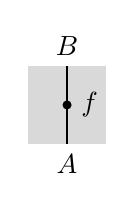
\begin{tikzpicture}[scale=0.5, baseline=($(bot)!0.5!(top)$)]
             %Coordinate layout and vertex positioning
            \path
                coordinate[label=below:\(A\)] (bot)
                +(0,1) coordinate[dot, label=right:\(f\)] (f)
                +(0,2) coordinate[label=above:\(B\)] (top);
            % Line drawing
            \draw (bot) -- (top);
            % Region filling
            \begin{scope}[on background layer]
            \fill[bg] (bot -| -1,0) rectangle (top -| 1,0);
            \end{scope}
        \end{tikzpicture}
        =
        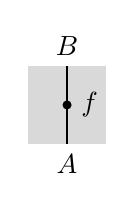
\begin{tikzpicture}[scale=0.5, baseline=($(bot)!0.5!(top)$)]
             %Coordinate layout and vertex positioning
            \path
                coordinate[label=below:\(A\)] (bot)
                +(0,1) coordinate[dot, label=right:\(f\)] (f)
                +(0,2) coordinate[label=above:\(B\)] (top);
            % Line drawing
            \draw (bot) -- (top);
            % Region filling
            \begin{scope}[on background layer]
            \fill[bg] (bot -| -1,0) rectangle (top -| 1,0);
            \end{scope}
        \end{tikzpicture}
        \circ
        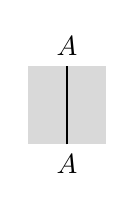
\begin{tikzpicture}[scale=0.5, baseline=($(bot)!0.5!(top)$)]
             %Coordinate layout and vertex positioning
            \path
                coordinate[label=below:\(A\)] (bot)
                +(0,1) coordinate[] (f)
                +(0,2) coordinate[label=above:\(A\)] (top);
            % Line drawing
            \draw (bot) -- (top);
            % Region filling
            \begin{scope}[on background layer]
            \fill[bg] (bot -| -1,0) rectangle (top -| 1,0);
            \end{scope}
        \end{tikzpicture}
    \end{equation*}

    \begin{equation*}
        
\begin{tikzpicture}[scale=0.5, baseline=($(bot)!0.5!(top)$)]
             %Coordinate layout and vertex positioning
            \path
                coordinate[] (bot)
                +(0,1) coordinate[] (f)
                +(0,2) coordinate[] (top);
            % Line drawing
            %\draw (bot) -- (top);
            % Region filling
            \begin{scope}[on background layer]
            \fill[bg] (bot -| -1,0) rectangle (top -| 1,0);
            \end{scope}
        \end{tikzpicture}
        \times
        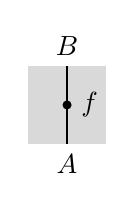
\begin{tikzpicture}[scale=0.5, baseline=($(bot)!0.5!(top)$)]
             %Coordinate layout and vertex positioning
            \path
                coordinate[label=below:\(A\)] (bot)
                +(0,1) coordinate[dot, label=right:\(f\)] (f)
                +(0,2) coordinate[label=above:\(B\)] (top);
            % Line drawing
            \draw (bot) -- (top);
            % Region filling
            \begin{scope}[on background layer]
            \fill[bg] (bot -| -1,0) rectangle (top -| 1,0);
            \end{scope}
        \end{tikzpicture}
        =
        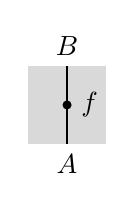
\begin{tikzpicture}[scale=0.5, baseline=($(bot)!0.5!(top)$)]
             %Coordinate layout and vertex positioning
            \path
                coordinate[label=below:\(A\)] (bot)
                +(0,1) coordinate[dot, label=right:\(f\)] (f)
                +(0,2) coordinate[label=above:\(B\)] (top);
            % Line drawing
            \draw (bot) -- (top);
            % Region filling
            \begin{scope}[on background layer]
            \fill[bg] (bot -| -1,0) rectangle (top -| 1,0);
            \end{scope}
        \end{tikzpicture}
        =
        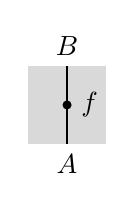
\begin{tikzpicture}[scale=0.5, baseline=($(bot)!0.5!(top)$)]
             %Coordinate layout and vertex positioning
            \path
                coordinate[label=below:\(A\)] (bot)
                +(0,1) coordinate[dot, label=right:\(f\)] (f)
                +(0,2) coordinate[label=above:\(B\)] (top);
            % Line drawing
            \draw (bot) -- (top);
            % Region filling
            \begin{scope}[on background layer]
            \fill[bg] (bot -| -1,0) rectangle (top -| 1,0);
            \end{scope}
        \end{tikzpicture}
        \times
        
\begin{tikzpicture}[scale=0.5, baseline=($(bot)!0.5!(top)$)]
             %Coordinate layout and vertex positioning
            \path
                coordinate[] (bot)
                +(0,1) coordinate[] (f)
                +(0,2) coordinate[] (top);
            % Line drawing
            %\draw (bot) -- (top);
            % Region filling
            \begin{scope}[on background layer]
            \fill[bg] (bot -| -1,0) rectangle (top -| 1,0);
            \end{scope}
        \end{tikzpicture}
    \end{equation*}

    \begin{equation*}
        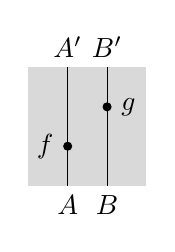
\begin{tikzpicture}[scale=0.5, baseline=($(dl)!0.5!(tl)$)]
             %Coordinate layout and vertex positioning
            \path
                coordinate[label=below:\(A\)] (dl)
                +(1,0)coordinate[label=below:\(B\)] (dr)
                +(0,1)coordinate[dot, label=left:\(f\)] (f)
                +(1,2)coordinate[dot, label=right:\(g\)] (g)
                +(0,3) coordinate[label=above:\(A'\)] (tl)
                +(1,3) coordinate[label=above:\(B'\)] (tr);
            % Line drawing
            \draw (dl) -- (tl);
            \draw (dr) -- (tr);
            % Region filling
            \begin{scope}[on background layer]
            \fill[bg] (dl -| -1,0) rectangle (tr -| 2,0);
            \end{scope}
        \end{tikzpicture}
        =
        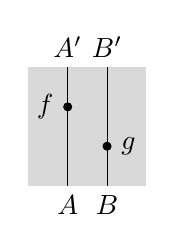
\begin{tikzpicture}[scale=0.5, baseline=($(dl)!0.5!(tl)$)]
             %Coordinate layout and vertex positioning
            \path
                coordinate[label=below:\(A\)] (dl)
                +(1,0)coordinate[label=below:\(B\)] (dr)
                +(0,2)coordinate[dot, label=left:\(f\)] (f)
                +(1,1)coordinate[dot, label=right:\(g\)] (g)
                +(0,3) coordinate[label=above:\(A'\)] (tl)
                +(1,3) coordinate[label=above:\(B'\)] (tr);
            % Line drawing
            \draw (dl) -- (tl);
            \draw (dr) -- (tr);
            % Region filling
            \begin{scope}[on background layer]
            \fill[bg] (dl -| -1,0) rectangle (tr -| 2,0);
            \end{scope}
        \end{tikzpicture}
    \end{equation*}
\end{frame}

\begin{frame}
    \frametitle{Multivalued functions}
    If \(f : A \times B \to C \times D \times E\) then we can draw it like so:
    \begin{center}
        \begin{tikzpicture}[scale=2]
             %Coordinate layout and vertex positioning
            \path
                coordinate[label=below:\(A\)] (dl)
                +(2,0) coordinate[label=below:\(B\)] (dr)
                +(1,1) coordinate[dot, label=below:\(f\)] (f)
                +(0,2) coordinate[label=above:\(C\)] (tl)
                +(1,2) coordinate[label=above:\(D\)] (top)
                +(2,2) coordinate[label=above:\(E\)] (tr);
            % Line drawing
            \draw (dl) to[out=90, in=180] (f) to[out=0, in=90] (dr);
            \draw (tl) to[out=-90, in=180] (f) to[out=0, in=-90] (tr);
            \draw (f) -- (top);
            % Region filling
            \begin{scope}[on background layer]
            \fill[bg] (bot -| -1,0) rectangle (tr -| 3,0);
            \end{scope}
        \end{tikzpicture}
    \end{center}
\end{frame}

\begin{frame}
    \frametitle{More constructs}
    \only<1-1>{
    Crossing over \((a, b) \mapsto (b, a)\):
    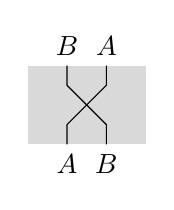
\begin{tikzpicture}[scale=0.5, baseline=($(dl)!0.5!(tl)$)]
         %Coordinate layout and vertex positioning
        \path
            coordinate[label=below:\(A\)] (dl)
            +(1,0) coordinate[label=below:\(B\)] (dr)
            +(0,0.5) coordinate[] (a)
            +(1,0.5) coordinate[] (b)
            +(0,1.5) coordinate[] (c)
            +(1,1.5) coordinate[] (d)
            +(0,2) coordinate[label=above:\(B\)] (tl)
            +(1,2) coordinate[label=above:\(A\)] (tr);
        % Line drawing
        \draw (dl) -- (a) -- (d) -- (tr);
        \draw (dr) -- (b) -- (c) -- (tl);
        % Region filling
        \begin{scope}[on background layer]
        \fill[bg] (dl -| -1,0) rectangle (tr -| 2,0);
        \end{scope}
    \end{tikzpicture},
    satisfying:

    \begin{equation*}
        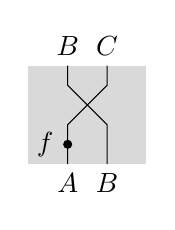
\begin{tikzpicture}[scale=0.5, baseline=($(dl)!0.5!(tl)$)]
             %Coordinate layout and vertex positioning
            \path
                coordinate[label=below:\(A\)] (dl)
                +(1,0) coordinate[label=below:\(B\)] (dr)
                +(0,0.5) coordinate[dot, label=left:\(f\)] (f)
                +(0,1) coordinate[] (a)
                +(1,1) coordinate[] (b)
                +(0,2) coordinate[] (c)
                +(1,2) coordinate[] (d)
                +(0,2.5) coordinate[label=above:\(B\)] (tl)
                +(1,2.5) coordinate[label=above:\(C\)] (tr);
            % Line drawing
            \draw (dl) -- (a) -- (d) -- (tr);
            \draw (dr) -- (b) -- (c) -- (tl);
            % Region filling
            \begin{scope}[on background layer]
            \fill[bg] (dl -| -1,0) rectangle (tr -| 2,0);
            \end{scope}
        \end{tikzpicture}
        =
        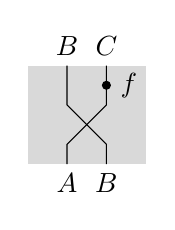
\begin{tikzpicture}[scale=0.5, baseline=($(dl)!0.5!(tl)$)]
             %Coordinate layout and vertex positioning
            \path
                coordinate[label=below:\(A\)] (dl)
                +(1,0) coordinate[label=below:\(B\)] (dr)
                +(0,0.5) coordinate[] (a)
                +(1,0.5) coordinate[] (b)
                +(0,1.5) coordinate[] (c)
                +(1,1.5) coordinate[] (d)
                +(1,2) coordinate[dot, label=right:\(f\)] (f)
                +(0,2.5) coordinate[label=above:\(B\)] (tl)
                +(1,2.5) coordinate[label=above:\(C\)] (tr);
            % Line drawing
            \draw (dl) -- (a) -- (d) -- (tr);
            \draw (dr) -- (b) -- (c) -- (tl);
            % Region filling
            \begin{scope}[on background layer]
            \fill[bg] (dl -| -1,0) rectangle (tr -| 2,0);
            \end{scope}
        \end{tikzpicture}
        \qquad
        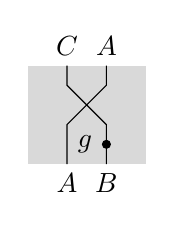
\begin{tikzpicture}[scale=0.5, baseline=($(dl)!0.5!(tl)$)]
             %Coordinate layout and vertex positioning
            \path
                coordinate[label=below:\(A\)] (dl)
                +(1,0) coordinate[label=below:\(B\)] (dr)
                +(1,0.5) coordinate[dot, label=left:\(g\)] (g)
                +(0,1) coordinate[] (a)
                +(1,1) coordinate[] (b)
                +(0,2) coordinate[] (c)
                +(1,2) coordinate[] (d)
                +(0,2.5) coordinate[label=above:\(C\)] (tl)
                +(1,2.5) coordinate[label=above:\(A\)] (tr);
            % Line drawing
            \draw (dl) -- (a) -- (d) -- (tr);
            \draw (dr) -- (b) -- (c) -- (tl);
            % Region filling
            \begin{scope}[on background layer]
            \fill[bg] (dl -| -1,0) rectangle (tr -| 2,0);
            \end{scope}
        \end{tikzpicture}
        =
        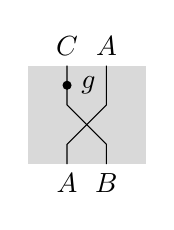
\begin{tikzpicture}[scale=0.5, baseline=($(dl)!0.5!(tl)$)]
             %Coordinate layout and vertex positioning
            \path
                coordinate[label=below:\(A\)] (dl)
                +(1,0) coordinate[label=below:\(B\)] (dr)
                +(0,0.5) coordinate[] (a)
                +(1,0.5) coordinate[] (b)
                +(0,1.5) coordinate[] (c)
                +(1,1.5) coordinate[] (d)
                +(0,2) coordinate[dot, label=right:\(g\)] (g)
                +(0,2.5) coordinate[label=above:\(C\)] (tl)
                +(1,2.5) coordinate[label=above:\(A\)] (tr);
            % Line drawing
            \draw (dl) -- (a) -- (d) -- (tr);
            \draw (dr) -- (b) -- (c) -- (tl);
            % Region filling
            \begin{scope}[on background layer]
            \fill[bg] (dl -| -1,0) rectangle (tr -| 2,0);
            \end{scope}
        \end{tikzpicture}
    \end{equation*}
    }

    \only<2-2>{
    Duplicating elements \(a \mapsto (a, a)\):
    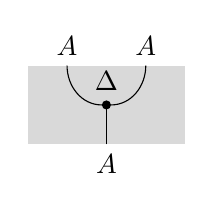
\begin{tikzpicture}[scale=0.5, baseline=($(bot)!0.5!(tl)$)]
         %Coordinate layout and vertex positioning
        \path
            coordinate[label=below:\(A\)] (bot)
            +(0,1)coordinate[dot, label=above:\(\Delta\)] (a)
            +(-1,2) coordinate[label=above:\(A\)] (tl)
            +(1,2) coordinate[label=above:\(A\)] (tr);
        % Line drawing
        \draw (bot) -- (a);
        \draw (tl) to[out=-90, in=180] (a) to[out=0, in=-90] (tr);
        % Region filling
        \begin{scope}[on background layer]
        \fill[bg] (bot -| -2,0) rectangle (tr -| 2,0);
        \end{scope}
    \end{tikzpicture},
    satisfying:

    \begin{equation*}
    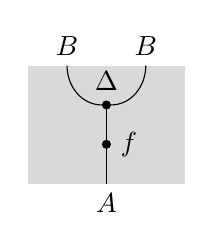
\begin{tikzpicture}[scale=0.5, baseline=($(bot)!0.5!(tl)$)]
         %coordinate layout and vertex positioning
        \path
            coordinate[label=below:\(A\)] (bot)
            +(0,1)coordinate[dot, label=right:\(f\)] (f)
            +(0,2)coordinate[dot, label=above:\(\Delta\)] (a)
            +(-1,3) coordinate[label=above:\(B\)] (tl)
            +(1,3) coordinate[label=above:\(B\)] (tr);
        % line drawing
        \draw (bot) -- (a);
        \draw (tl) to[out=-90, in=180] (a) to[out=0, in=-90] (tr);
        % region filling
        \begin{scope}[on background layer]
        \fill[bg] (bot -| -2,0) rectangle (tr -| 2,0);
        \end{scope}
    \end{tikzpicture}
    =
    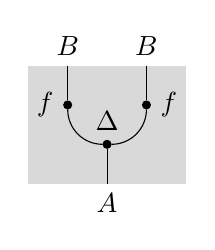
\begin{tikzpicture}[scale=0.5, baseline=($(bot)!0.5!(tl)$)]
         %coordinate layout and vertex positioning
        \path
            coordinate[label=below:\(A\)] (bot)
            +(0,1)coordinate[dot, label=above:\(\Delta\)] (a)
            +(-1,2) coordinate[dot, label=left:\(f\)] (b)
            +(1,2) coordinate[dot, label=right:\(f\)] (c)
            +(-1,3)coordinate[label=above:\(B\)] (tl)
            +(1,3)coordinate[label=above:\(B\)] (tr);
        % line drawing
        \draw (bot) -- (a);
        \draw (b) to[out=-90, in=180] (a) to[out=0, in=-90] (c);
        \draw (b) -- (tl);
        \draw (c) -- (tr);
        % region filling
        \begin{scope}[on background layer]
        \fill[bg] (bot -| -2,0) rectangle (tr -| 2,0);
        \end{scope}
    \end{tikzpicture}
    \end{equation*}

    \begin{equation*}
    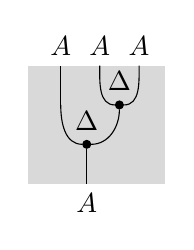
\begin{tikzpicture}[scale=0.5, baseline=($(bot)!0.5!(tl)$)]
         %coordinate layout and vertex positioning
        \path
            coordinate[label=below:\(A\)] (bot)
            +(0,1)coordinate[dot, label=above:\(\Delta\)] (a)
            +(-0.66,2)coordinate[] (b)
            +(0.83,2)coordinate[dot, label=above:\(\Delta\)] (c)
            +(-0.66,3) coordinate[label=above:\(A\)] (tl)
            +(0.33,3) coordinate[label=above:\(A\)] (top)
            +(1.33,3) coordinate[label=above:\(A\)] (tr);
        % line drawing
        \draw (bot) -- (a);
        \draw (b) to[out=-90, in=180] (a) to[out=0, in=-90] (c);
        \draw (b) -- (tl);
        \draw (top) to[out=-90, in=180] (c) to[out=0, in=-90] (tr);
        % region filling
        \begin{scope}[on background layer]
        \fill[bg] (bot -| -1.5,0) rectangle (tr -| 2,0);
        \end{scope}
    \end{tikzpicture}
    =
    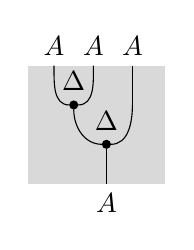
\begin{tikzpicture}[scale=0.5, baseline=($(bot)!0.5!(tl)$)]
         %coordinate layout and vertex positioning
        \path
            coordinate[label=below:\(A\)] (bot)
            +(0,1)coordinate[dot, label=above:\(\Delta\)] (a)
            +(-0.83,2)coordinate[dot, label=above:\(\Delta\)] (b)
            +(0.66,2)coordinate[] (c)
            +(-1.33,3) coordinate[label=above:\(A\)] (tl)
            +(-0.33,3) coordinate[label=above:\(A\)] (top)
            +(0.66,3) coordinate[label=above:\(A\)] (tr);
        % line drawing
        \draw (bot) -- (a);
        \draw (b) to[out=-90, in=180] (a) to[out=0, in=-90] (c);
        \draw (tl) to[out=-90, in=180] (b) to[out=0, in=-90] (top);
        \draw (c) -- (tr);
        % region filling
        \begin{scope}[on background layer]
        \fill[bg] (bot -| -2,0) rectangle (tr -| 1.5,0);
        \end{scope}
    \end{tikzpicture}
    \end{equation*}
    }

    \only<3-3>{
    Deleting elements:
    \begin{tikzpicture}[scale=0.5, baseline=($(bot)!0.5!(top)$)]
         %Coordinate layout and vertex positioning
        \path
            coordinate[label=below:\(A\)] (bot)
            +(0,1)coordinate[dot] (a)
            +(0,2) coordinate[] (top);
        % Line drawing
        \draw (bot) -- (a);
        % Region filling
        \begin{scope}[on background layer]
        \fill[bg] (bot -| -2,0) rectangle (tr -| 2,0);
        \end{scope}
    \end{tikzpicture},
    satisfying:

    \begin{equation*}
    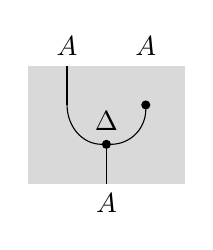
\begin{tikzpicture}[scale=0.5, baseline=($(bot)!0.5!(tl)$)]
         %coordinate layout and vertex positioning
        \path
            coordinate[label=below:\(A\)] (bot)
            +(0,1)coordinate[dot, label=above:\(\Delta\)] (a)
            +(-1,2)coordinate[] (b)
            +(1,2)coordinate[dot] (c)
            +(-1,3) coordinate[label=above:\(A\)] (tl)
            +(1,3) coordinate[label=above:\(A\)] (tr);
        % line drawing
        \draw (bot) -- (a);
        \draw (b) to[out=-90, in=180] (a) to[out=0, in=-90] (c);
        \draw (b) -- (tl);
        % region filling
        \begin{scope}[on background layer]
        \fill[bg] (bot -| -2,0) rectangle (tr -| 2,0);
        \end{scope}
    \end{tikzpicture}
    =
    \begin{tikzpicture}[scale=0.5, baseline=($(bot)!0.5!(top)$)]
         %coordinate layout and vertex positioning
        \path
            coordinate[label=below:\(A\)] (bot)
            +(0,1)coordinate[] (a)
            +(0,2)coordinate[] (b)
            +(0,3) coordinate[label=above:\(A\)] (top);
        % line drawing
        \draw (bot) -- (top);
        % region filling
        \begin{scope}[on background layer]
        \fill[bg] (bot -| -2,0) rectangle (tr -| 2,0);
        \end{scope}
    \end{tikzpicture}
    =
    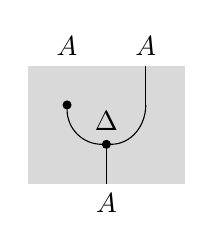
\begin{tikzpicture}[scale=0.5, baseline=($(bot)!0.5!(tl)$)]
         %coordinate layout and vertex positioning
        \path
            coordinate[label=below:\(A\)] (bot)
            +(0,1)coordinate[dot, label=above:\(\Delta\)] (a)
            +(-1,2)coordinate[dot] (b)
            +(1,2)coordinate[] (c)
            +(-1,3) coordinate[label=above:\(A\)] (tl)
            +(1,3) coordinate[label=above:\(A\)] (tr);
        % line drawing
        \draw (bot) -- (a);
        \draw (b) to[out=-90, in=180] (a) to[out=0, in=-90] (c);
        \draw (c) -- (tr);
        % region filling
        \begin{scope}[on background layer]
        \fill[bg] (bot -| -2,0) rectangle (tr -| 2,0);
        \end{scope}
    \end{tikzpicture}
    \end{equation*}
    }
\end{frame}

\section{Worked example: monoid algebra}

\begin{frame}
    \frametitle{Monoids}
    \begin{definition}
        A monoid is a set \(M\) equipped with a multiplication \(\mu : M \times M \to M\) (we write \(\mu(a, b) = a * b\)) and an element \(e \in M\) called the identity satisfying:
        \begin{itemize}
            \item (associativity) for any \(a, b, c \in M\), \(a * (b * c) = (a * b) * c\),
            \item (identity) for any \(a \in M\), \(e * a = a = a * e\).
        \end{itemize}
    \end{definition}
    \pause
    \begin{example}
        \begin{itemize}
            \item The natural numbers under addition \((\NN, +, 0)\)
            \item The natural numbers under multiplication \((\NN, *, 1)\)
            \item Matrices under multiplication \((\mathrm{Mat}_n, *, I_n)\)
            \item Strings under concatenation \((A^*, ||, )\)
        \end{itemize}
    \end{example}
\end{frame}

\begin{frame}
    \frametitle{Monoids diagramatically}
    The map \(\mu : M \times M \to M\) and element \(e \in M\) satisfy:

    Associativity:
    \begin{equation*}
        \begin{tikzpicture}[scale=0.5, baseline=($(bot)!0.5!(tl)$)]
             %Coordinate layout and vertex positioning
            \path
                coordinate[label=below:\(M\)] (bot)
                +(-1,0) coordinate[label=below:\(M\)] (dl)
                +(1,0) coordinate[label=below:\(M\)] (dr)
                +(-0.5,1) coordinate[dot, label=below:\(\mu\)] (a)
                +(1,1) coordinate[] (b)
                +(0.33,2) coordinate[dot, label=below:\(\mu\)] (c)
                +(0.33,3) coordinate[label=above:\(M\)] (top);
            % Line drawing
            \draw (dr) -- (b);
            \draw (dl) to[out=90, in=180] (a) to[out=0, in=90] (bot);
            \draw (a) to[out=90, in=180] (c) to[out=0, in=90] (b);
            \draw (c) -- (top);
            % Region filling
            \begin{scope}[on background layer]
            \fill[bg] (bot -| -2,0) rectangle (top -| 2,0);
            \end{scope}
        \end{tikzpicture}
        =
        \begin{tikzpicture}[scale=0.5, baseline=($(bot)!0.5!(tl)$)]
             %Coordinate layout and vertex positioning
            \path
                coordinate[label=below:\(M\)] (bot)
                +(-1,0) coordinate[label=below:\(M\)] (dl)
                +(1,0) coordinate[label=below:\(M\)] (dr)
                +(-1,1) coordinate[] (b)
                +(0.5,1) coordinate[dot, label=below:\(\mu\)] (a)
                +(-0.33,2) coordinate[dot, label=below:\(\mu\)] (c)
                +(-0.33,3) coordinate[label=above:\(M\)] (top);
            % Line drawing
            \draw (dl) -- (b);
            \draw (bot) to[out=90, in=180] (a) to[out=0, in=90] (dr);
            \draw (b) to[out=90, in=180] (c) to[out=0, in=90] (a);
            \draw (c) -- (top);
            % Region filling
            \begin{scope}[on background layer]
            \fill[bg] (bot -| -2,0) rectangle (top -| 2,0);
            \end{scope}
        \end{tikzpicture}
    \end{equation*}

    Identity:
    \begin{equation*}
        \begin{tikzpicture}[scale=0.5, baseline=($(bot)!0.5!(tl)$)]
             %Coordinate layout and vertex positioning
            \path
                coordinate[label=below:\(M\)] (bot)
                +(0,1) coordinate[] (a)
                +(1,1) coordinate[dot, label=below:\(e\)] (b)
                +(0.5,2) coordinate[dot, label=below:\(\mu\)] (c)
                +(0.5,3) coordinate[label=above:\(M\)] (top);
            % Line drawing
            \draw (bot) -- (a);
            \draw (a) to[out=90, in=180] (c) to[out=0, in=90] (b);
            \draw (c) -- (top);
            % Region filling
            \begin{scope}[on background layer]
            \fill[bg] (bot -| -1,0) rectangle (top -| 2,0);
            \end{scope}
        \end{tikzpicture}
        =
        \begin{tikzpicture}[scale=0.5, baseline=($(bot)!0.5!(tl)$)]
             %Coordinate layout and vertex positioning
            \path
                coordinate[label=below:\(M\)] (bot)
                +(0,1) coordinate[] (a)
                +(0,1) coordinate[] (b)
                +(0,2) coordinate[] (c)
                +(0,3) coordinate[label=above:\(M\)] (top);
            % Line drawing
            \draw (bot) -- (top);
            % Region filling
            \begin{scope}[on background layer]
            \fill[bg] (bot -| -1,0) rectangle (top -| 1,0);
            \end{scope}
        \end{tikzpicture}
        =
        \begin{tikzpicture}[scale=0.5, baseline=($(bot)!0.5!(tl)$)]
             %Coordinate layout and vertex positioning
            \path
                coordinate[label=below:\(M\)] (bot)
                +(0,1) coordinate[] (a)
                +(-1,1) coordinate[dot, label=below:\(e\)] (b)
                +(-0.5,2) coordinate[dot, label=below:\(\mu\)] (c)
                +(-0.5,3) coordinate[label=above:\(M\)] (top);
            % Line drawing
            \draw (bot) -- (a);
            \draw (b) to[out=90, in=180] (c) to[out=0, in=90] (a);
            \draw (c) -- (top);
            % Region filling
            \begin{scope}[on background layer]
            \fill[bg] (bot -| -2,0) rectangle (top -| 1,0);
            \end{scope}
        \end{tikzpicture}
    \end{equation*}
\end{frame}

\begin{frame}
    \frametitle{Product monoid}
    \only<-6>{
    Let \((M, \mu, e), (M', \mu', e')\) be monoids.
    Define the product monoid, with set \(M \times M'\) as follows.

    \pause
    Identity:

    \begin{equation*}
        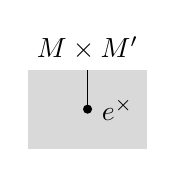
\begin{tikzpicture}[scale=0.5, baseline=($(bot)!0.5!(top)$)]
             %Coordinate layout and vertex positioning
            \path
                coordinate[] (bot)
                +(0, 1) coordinate[dot, label=right:\(e^\times\)] (a)
                +(0, 2) coordinate[label=above:\(M \times M'\)] (top);
            % Line drawing
            \draw (a) -- (top);
            % Region filling
            \begin{scope}[on background layer]
            \fill[bg] (bot -| -1.5,0) rectangle (top -| 1.5,0);
            \end{scope}
        \end{tikzpicture}
        :=
        \only<2-2>{
        \begin{tikzpicture}[scale=0.5, baseline=($(bot)!0.5!(tl)$)]
             %Coordinate layout and vertex positioning
            \path
                coordinate[] (bot)
                +(0,1) coordinate[] (a)
                +(1,1) coordinate[] (b)
                +(0,2) coordinate[label=above:\(M\)] (tl)
                +(1,2) coordinate[label=above:\(M'\)] (tr);
            % Line drawing
            % Region filling
            \begin{scope}[on background layer]
            \fill[bg] (bot -| -1,0) rectangle (top -| 2,0);
            \end{scope}
        \end{tikzpicture}
        }
        \only<3->{
        \begin{tikzpicture}[scale=0.5, baseline=($(bot)!0.5!(tl)$)]
             %Coordinate layout and vertex positioning
            \path
                coordinate[] (bot)
                +(0,1) coordinate[dot, blue, label=left:\(e\)] (a)
                +(1,1) coordinate[dot, red, label=right:\(e'\)] (b)
                +(0,2) coordinate[label=above:\(M\)] (tl)
                +(1,2) coordinate[label=above:\(M'\)] (tr);
            % Line drawing
            \draw[blue] (a) -- (tl);
            \draw[red] (b) -- (tr);
            % Region filling
            \begin{scope}[on background layer]
            \fill[bg] (bot -| -1,0) rectangle (top -| 2,0);
            \end{scope}
        \end{tikzpicture}
        }
    \end{equation*}

    \pause[4]
    Multiplication:

    \begin{equation*}
        \begin{tikzpicture}[scale=0.5, baseline=($(dl)!0.5!(tl)$)]
             %Coordinate layout and vertex positioning
            \path
                coordinate[label=below:\(M \times M'\)] (dl)
                +(3,0) coordinate[label=below:\(M \times M'\)] (dr)
                +(1.5,2) coordinate[dot, label=below:\(\mu^\times\)] (a)
                +(1.5,3) coordinate[label=above:\(M \times M'\)] (top);
            % Line drawing
            \draw (dl) to[out=90, in=180] (a) to[out=0, in=90] (dr);
            \draw (a) -- (top);
            % Region filling
            \begin{scope}[on background layer]
            \fill[bg] (bot -| -1,0) rectangle (top -| 4,0);
            \end{scope}
        \end{tikzpicture}
        :=
        \only<4-4>{
        \begin{tikzpicture}[scale=0.5, baseline=($(dl)!0.5!(tl)$)]
             %Coordinate layout and vertex positioning
            \path
                coordinate[label=below:\(M\)] (dll)
                +(1,0) coordinate[label=below:\(M'\)] (dl)
                +(2,0) coordinate[label=below:\(M\)] (dr)
                +(3,0) coordinate[label=below:\(M'\)] (drr)
                +(1,1) coordinate[] (a)
                +(2,1) coordinate[] (b)
                +(1,2) coordinate[label=above:\(M\)] (tl)
                +(2,2) coordinate[label=above:\(M'\)] (tr);
            % Line drawing
            % Region filling
            \begin{scope}[on background layer]
            \fill[bg] (bot -| -1,0) rectangle (tr -| 4,0);
            \end{scope}
        \end{tikzpicture}
        }
        \only<5-5>{
        \begin{tikzpicture}[scale=0.5, baseline=($(dl)!0.5!(tl)$)]
             %Coordinate layout and vertex positioning
            \path
                coordinate[label=below:\(M\)] (dll)
                +(1,0) coordinate[label=below:\(M'\)] (dl)
                +(2,0) coordinate[label=below:\(M\)] (dr)
                +(3,0) coordinate[label=below:\(M'\)] (drr)
                +(1,1) coordinate[dot, blue, label=135:\(\mu\)] (a)
                +(2,1) coordinate[] (b)
                +(1,2) coordinate[label=above:\(M\)] (tl)
                +(2,2) coordinate[label=above:\(M'\)] (tr);
            % Line drawing
            \draw[blue] (dll) to[out=90, in=180] (a) to[out=0, in=90] (dr);
            \draw[blue] (a) -- (tl);
            % Region filling
            \begin{scope}[on background layer]
            \fill[bg] (bot -| -1,0) rectangle (tr -| 4,0);
            \end{scope}
        \end{tikzpicture}
        }
        \only<6-6>{
        \begin{tikzpicture}[scale=0.5, baseline=($(dl)!0.5!(tl)$)]
             %Coordinate layout and vertex positioning
            \path
                coordinate[label=below:\(M\)] (dll)
                +(1,0) coordinate[label=below:\(M'\)] (dl)
                +(2,0) coordinate[label=below:\(M\)] (dr)
                +(3,0) coordinate[label=below:\(M'\)] (drr)
                +(1,1) coordinate[dot, blue, label=135:\(\mu\)] (a)
                +(2,1) coordinate[dot, red, label=45:\(\mu'\)] (b)
                +(1,2) coordinate[label=above:\(M\)] (tl)
                +(2,2) coordinate[label=above:\(M'\)] (tr);
            % Line drawing
            \draw[blue] (dll) to[out=90, in=180] (a) to[out=0, in=90] (dr);
            \draw[red] (dl) to[out=90, in=180] (b) to[out=0, in=90] (drr);
            \draw[blue] (a) -- (tl);
            \draw[red] (b) -- (tr);
            % Region filling
            \begin{scope}[on background layer]
            \fill[bg] (bot -| -1,0) rectangle (tr -| 4,0);
            \end{scope}
        \end{tikzpicture}
        }
    \end{equation*}
    }
    \only<7-10>{
        Left identity:
        \begin{align*}
        \begin{tikzpicture}[scale=0.5, baseline=($(dl)!0.5!(tl)$)]
             %Coordinate layout and vertex positioning
            \path
                coordinate[label=below:\(M \times M'\)] (dl)
                +(0, 0.5) coordinate[dot, label=left:\(e^\times\)] (a)
                +(3,0) coordinate[label=below:\(M \times M'\)] (dr)
                +(1.5,2) coordinate[dot, label=below:\(\mu^\times\)] (b)
                +(3,0.5) coordinate[] (c)
                +(1.5,3) coordinate[label=above:\(M \times M'\)] (top);
            % Line drawing
            \draw (a) to[out=90, in=180] (b) to[out=0, in=90] (c);
            \draw (b) -- (top);
            \draw (dr) -- (c);
            % Region filling
            \begin{scope}[on background layer]
            \fill[bg] (bot -| -1,0) rectangle (top -| 4,0);
            \end{scope}
        \end{tikzpicture}
        \uncover<8->{
        &=
        \begin{tikzpicture}[scale=0.5, baseline=($(dl)!0.5!(tl)$)]
             %Coordinate layout and vertex positioning
            \path
                coordinate[] (dll)
                +(1,0) coordinate[] (dl)
                +(0,1) coordinate[dot, blue, label=below:\(e\)] (a)
                +(1,1) coordinate[dot, red, label=below:\(e'\)] (b)
                +(2,0) coordinate[label=below:\(M\)] (dr)
                +(3,0) coordinate[label=below:\(M'\)] (drr)
                +(2,1) coordinate[] (c)
                +(3,1) coordinate[] (d)
                +(1,2) coordinate[dot, blue, label=135:\(\mu\)] (e)
                +(2,2) coordinate[dot, red, label=45:\(\mu'\)] (f)
                +(1,3) coordinate[label=above:\(M\)] (tl)
                +(2,3) coordinate[label=above:\(M'\)] (tr);
            % Line drawing
            \draw[blue] (a) to[out=90, in=180] (e) to[out=0, in=90] (c);
            \draw[red] (b) to[out=90, in=180] (f) to[out=0, in=90] (d);
            \draw[blue] (dr) -- (c);
            \draw[red] (drr) -- (d);
            \draw[blue] (e) -- (tl);
            \draw[red] (f) -- (tr);
            % Region filling
            \begin{scope}[on background layer]
            \fill[bg] (bot -| -1,0) rectangle (tr -| 4,0);
            \end{scope}
        \end{tikzpicture}
        \uncover<9->{
        =
        \begin{tikzpicture}[scale=0.5, baseline=($(dl)!0.5!(tl)$)]
             %Coordinate layout and vertex positioning
            \path
                coordinate[] (dll)
                +(1,0) coordinate[] (dl)
                +(0,1) coordinate[dot, blue, label=below:\(e\)] (a)
                +(1.8,1) coordinate[dot, red, label=below:\(e'\)] (b)
                +(1.5,0) coordinate[label=below:\(M\)] (dr)
                +(3,0) coordinate[label=below:\(M'\)] (drr)
                +(1.5,1) coordinate[] (c)
                +(3,1) coordinate[] (d)
                +(1,2) coordinate[dot, blue, label=135:\(\mu\)] (e)
                +(2,2) coordinate[dot, red, label=45:\(\mu'\)] (f)
                +(1,3) coordinate[label=above:\(M\)] (tl)
                +(2,3) coordinate[label=above:\(M'\)] (tr);
            % Line drawing
            \draw[blue] (a) to[out=90, in=180] (e) to[out=0, in=90] (c);
            \draw[red] (b) to[out=90, in=225] (f) to[out=0, in=90] (d);
            \draw[blue] (dr) -- (c);
            \draw[red] (drr) -- (d);
            \draw[blue] (e) -- (tl);
            \draw[red] (f) -- (tr);
            % Region filling
            \begin{scope}[on background layer]
            \fill[bg] (bot -| -1,0) rectangle (tr -| 4,0);
            \end{scope}
        \end{tikzpicture}\\
        &=
        }
        \begin{tikzpicture}[scale=0.5, baseline=($(dl)!0.5!(tl)$)]
             %Coordinate layout and vertex positioning
            \path
                coordinate[label=below:\(M\)] (dl)
                +(1,0) coordinate[label=below:\(M'\)] (dr)
                +(0,3) coordinate[label=above:\(M\)] (tl)
                +(1,3) coordinate[label=above:\(M'\)] (tr);
            % Line drawing
            \draw[blue] (dl) -- (tl);
            \draw[red] (dr) -- (tr);
            % Region filling
            \begin{scope}[on background layer]
            \fill[bg] (bot -| -1,0) rectangle (tr -| 2,0);
            \end{scope}
        \end{tikzpicture}
        =
        }
        \begin{tikzpicture}[scale=0.5, baseline=($(bot)!0.5!(top)$)]
             %Coordinate layout and vertex positioning
            \path
                coordinate[label=below:\(M \times M'\)] (bot)
                +(0,3) coordinate[label=above:\(M \times M'\)] (top);
            % Line drawing
            \draw (bot) -- (top);
            % Region filling
            \begin{scope}[on background layer]
            \fill[bg] (bot -| -1,0) rectangle (tr -| 1,0);
            \end{scope}
        \end{tikzpicture}
        \end{align*}
        \uncover<10->{
        Right identity is similar.
        }
    }
    \only<11->{
        Associativity:
        \begin{align*}
        \begin{tikzpicture}[scale=0.5, baseline=($(bot)!0.5!(tl)$)]
             %Coordinate layout and vertex positioning
            \path
                coordinate[] (bot)
                +(-1,0) coordinate[] (dl)
                +(1,0) coordinate[] (dr)
                +(-0.5,1) coordinate[dot, label=below:\(\mu^\times\)] (a)
                +(1,1) coordinate[] (b)
                +(0.33,2) coordinate[dot, label=below:\(\mu^\times\)] (c)
                +(0.33,3) coordinate[] (top);
            % Line drawing
            \draw (dr) -- (b);
            \draw (dl) to[out=90, in=180] (a) to[out=0, in=90] (bot);
            \draw (a) to[out=90, in=180] (c) to[out=0, in=90] (b);
            \draw (c) -- (top);
            % Region filling
            \begin{scope}[on background layer]
            \fill[bg] (bot -| -2,0) rectangle (top -| 2,0);
            \end{scope}
        \end{tikzpicture}
        \uncover<12->{
        &=
        \begin{tikzpicture}[scale=0.5, baseline=($(dl)!0.5!(tl)$)]
             %Coordinate layout and vertex positioning
            \path
                coordinate[] (dlll)
                +(1,0) coordinate[] (dll)
                +(2,0) coordinate[] (dl)
                +(3,0) coordinate[] (dr)
                +(4,0) coordinate[] (drr)
                +(5,0) coordinate[] (drrr)
                +(1,1) coordinate[dot, blue] (a)
                +(2,1) coordinate[dot, red] (b)
                +(4,1) coordinate[] (c)
                +(5,1) coordinate[] (d)
                +(2.5,2) coordinate[dot, blue] (e)
                +(3.5,2) coordinate[dot, red] (f)
                +(2.5,3) coordinate[] (tl)
                +(3.5,3) coordinate[] (tr);
            % Line drawing
            \draw[blue] (dlll) to[out=90, in=180] (a) to[out=0, in=90] (dl);
            \draw[red] (dll) to[out=90, in=180] (b) to[out=0, in=90] (dr);
            \draw[blue] (a) to[out=90, in=190] (e) to[out=-10, in=90] (c);
            \draw[red] (b) to[out=90, in=190] (f) to[out=-10, in=90] (d);
            \draw[blue] (drr) -- (c);
            \draw[red] (drrr) -- (d);
            \draw[blue] (e) -- (tl);
            \draw[red] (f) -- (tr);
            % Region filling
            \begin{scope}[on background layer]
            \fill[bg] (bot -| -1,0) rectangle (tr -| 6,0);
            \end{scope}
        \end{tikzpicture}\\
        \uncover<13->{
        &=
        \begin{tikzpicture}[scale=0.5, baseline=($(dl)!0.5!(tl)$)]
             %Coordinate layout and vertex positioning
            \path
                coordinate[] (dlll)
                +(1,0) coordinate[] (dll)
                +(2,0) coordinate[] (dl)
                +(3,0) coordinate[] (dr)
                +(4,0) coordinate[] (drr)
                +(5,0) coordinate[] (drrr)
                +(1,1) coordinate[dot, blue] (a)
                +(3,1.5) coordinate[dot, red] (b)
                +(5,1) coordinate[] (d)
                +(1.5,1.5) coordinate[dot, blue] (e)
                +(3.5,2) coordinate[dot, red] (f)
                +(1.5,3) coordinate[] (tl)
                +(3.5,3) coordinate[] (tr);
            % Line drawing
            \draw[blue] (dlll) to[out=90, in=180] (a) to[out=0, in=90] (dl);
            \draw[red] (dll) to[out=90, in=180] (b) to[out=0, in=90] (dr);
            \draw[blue] (a) to[out=90, in=190] (e) to[out=-10, in=90] (drr);
            \draw[red] (b) to[out=90, in=190] (f) to[out=-10, in=90] (d);
            \draw[red] (drrr) -- (d);
            \draw[blue] (e) -- (tl);
            \draw[red] (f) -- (tr);
            % Region filling
            \begin{scope}[on background layer]
            \fill[bg] (bot -| -1,0) rectangle (tr -| 6,0);
            \end{scope}
        \end{tikzpicture}
        \uncover<14->{
        =
        \begin{tikzpicture}[scale=0.5, baseline=($(dl)!0.5!(tl)$)]
             %Coordinate layout and vertex positioning
            \path
                coordinate[] (dlll)
                +(1,0) coordinate[] (dll)
                +(2,0) coordinate[] (dl)
                +(3,0) coordinate[] (dr)
                +(4,0) coordinate[] (drr)
                +(5,0) coordinate[] (drrr)
                +(1,1) coordinate[] (a)
                +(3,1.5) coordinate[] (b)
                +(5,1) coordinate[] (d)
                +(1.5,1.5) coordinate[dot, blue] (e)
                +(3.5,1.5) coordinate[dot, red] (f)
                +(1,2) coordinate[dot, blue] (g)
                +(3,2) coordinate[dot, red] (h)
                +(1,3) coordinate[] (tl)
                +(3,3) coordinate[] (tr);
            % Line drawing
            \draw[blue] (dl) to (a) to[out=90, in=190] (e) to[out=-10, in=90] (drr);
            \draw[red] (dr) to[out=90, in=180] (f) to[out=0, in=90] (drrr);
            \draw[blue] (dlll) to[out=90, in=180] (g) to[out=0, in=90] (e);
            \draw[red] (dll) to[out=75, in=190] (h) to[out=-10, in=90] (f);
            \draw[blue] (g) -- (tl);
            \draw[red] (h) -- (tr);
            % Region filling
            \begin{scope}[on background layer]
            \fill[bg] (bot -| -1,0) rectangle (tr -| 6,0);
            \end{scope}
        \end{tikzpicture}\\
        \uncover<15->{
        &=
        \begin{tikzpicture}[scale=0.5, baseline=($(dl)!0.5!(tl)$)]
             %Coordinate layout and vertex positioning
            \path
                coordinate[] (dlll)
                +(1,0) coordinate[] (dll)
                +(2,0) coordinate[] (dl)
                +(3,0) coordinate[] (dr)
                +(4,0) coordinate[] (drr)
                +(5,0) coordinate[] (drrr)
                +(0,1) coordinate[] (a)
                +(1,1) coordinate[] (b)
                +(3,1) coordinate[dot, blue] (c)
                +(4,1) coordinate[dot, red] (d)
                +(1.5,2) coordinate[dot, blue] (e)
                +(2.5,2) coordinate[dot, red] (f)
                +(1.5,3) coordinate[] (tl)
                +(2.5,3) coordinate[] (tr);
            % Line drawing
            \draw[blue] (dl) to[out=90, in=180] (c) to[out=0, in=90] (drr);
            \draw[red] (dr) to[out=90, in=180] (d) to[out=0, in=90] (drrr);
            \draw[blue] (a) to[out=90, in=190] (e) to[out=-10, in=90] (c);
            \draw[red] (b) to[out=90, in=190] (f) to[out=-10, in=90] (d);
            \draw[blue] (dlll) -- (a);
            \draw[red] (dll) -- (b);
            \draw[blue] (e) -- (tl);
            \draw[red] (f) -- (tr);
            % Region filling
            \begin{scope}[on background layer]
            \fill[bg] (bot -| -1,0) rectangle (tr -| 6,0);
            \end{scope}
        \end{tikzpicture}
        =
        }}}}
        \begin{tikzpicture}[scale=0.5, baseline=($(bot)!0.5!(tl)$)]
             %Coordinate layout and vertex positioning
            \path
                coordinate[] (bot)
                +(-1,0) coordinate[] (dl)
                +(1,0) coordinate[] (dr)
                +(-1,1) coordinate[] (b)
                +(0.5,1) coordinate[dot, label=below:\(\mu^\times\)] (a)
                +(-0.33,2) coordinate[dot, label=below:\(\mu^\times\)] (c)
                +(-0.33,3) coordinate[] (top);
            % Line drawing
            \draw (dl) -- (b);
            \draw (bot) to[out=90, in=180] (a) to[out=0, in=90] (dr);
            \draw (b) to[out=90, in=180] (c) to[out=0, in=90] (a);
            \draw (c) -- (top);
            % Region filling
            \begin{scope}[on background layer]
            \fill[bg] (bot -| -2,0) rectangle (top -| 2,0);
            \end{scope}
        \end{tikzpicture}
        \end{align*}
    }
\end{frame}

\end{document}
